\documentclass[a4paper,10pt]{article}
\usepackage[utf8]{inputenc}
\usepackage[T1]{fontenc}
\usepackage[ngerman]{babel}
\usepackage{CJKutf8}
\usepackage{graphicx}
\pagestyle{plain}

\title{Shigatsu wa Kimi no Uso}
\author{Naoshi Arakawa}
\date{2016}

\begin{document}

\maketitle

\begin{figure}[h]
\begin{center}
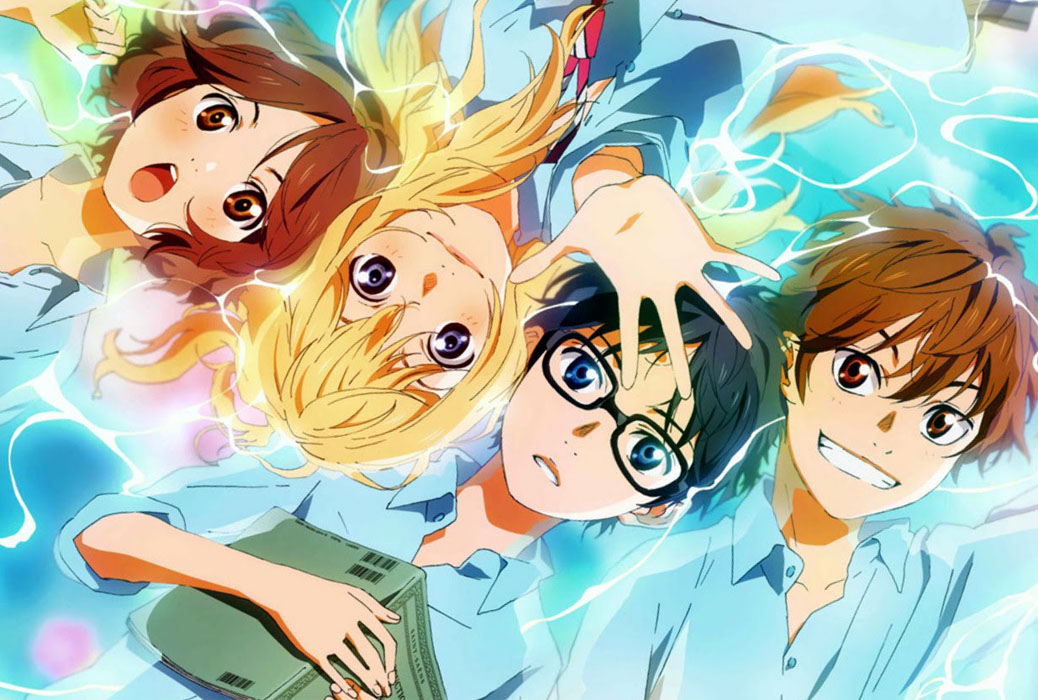
\includegraphics[width=4cm]{YLIA.jpg}
\end{center}
\end{figure}

\begin{CJK}{UTF8}{min}

\section{Your Lie in April}
Your Lie in April, known in Japan as Shigatsu wa Kimi no Uso (四月は君の嘘)\\
or just simply Kimiuso, is a Japanese manga series written and illustrated by Naoshi Arakawa. The series was serialized in Kodansha's Monthly Shōnen Magazine from April 2011 to May 2015. An anime television series adaptation by A-1 Pictures aired from October 2014 to March 2015 on Fuji TV's Noitamina block.[4] A live-action film adaptation of the same name was released in September 2016.\\
\subsection{Anime television series}
\begin{table}[h]
\begin{tabular}{r|l}

\textbf{Directed by}      & Kyōhei Ishiguro\\\\
\textbf{Written by}       & Takao Yoshioka\\\\
\textbf{Music by}         & Masaru Yokoyama\\\\
\textbf{Studio}           &  	A-1 Pictures\\\\
\textbf{Original network} & Fuji TV (Noitamina\\\\
\textbf{Original run}     & October 9, 2014 – March 19, 2015\\\\
\textbf{Episodes}         & 22 (List of episodes)

\end{tabular}
\end{table}

\newpage
\subsection{Plot}
Piano prodigy Kōsei Arima dominated various music competitions and has become famous among child musicians but also controversial. After his mother, who was also his coldhearted, abusive instructor who forced him to play the piano emotionlessly, died, he had a mental breakdown while performing at a piano recital at the age of eleven. As a result, he is no longer able to hear the sound of his piano even though his hearing is perfectly fine.

Two years later, Kōsei hasn't touched the piano and views the world in monochrome, without any flair or color, resigning himself to living out his life with his good friends, Tsubaki and Watari, until, one day, a girl changes everything. Kaori Miyazono, an audacious, free-spirited, fourteen-year-old violinist whose playing style reflects her manic personality, helps Kōsei return to the music world and shows that it should be free and mold-breaking unlike the structured and rigid style Kōsei was used to, and as she continues to uplift him, he quickly realizes that he loves her, though she already likes Watari.

However, while performing together (Kōsei having been dragged into it by Kaori), Kaori suddenly collapses after a moving performance and is hospitalised. At first Kaori says that she is anaemic and just needs some routine testing, but this is revealed to be a lie when flashes of her past reveal her collapsing and bleeding many times before.

Finally Kaori is discharged and back to her happy, crazy-self, inviting Kōsei to play at a Gala with her. However, Kaori fails to show up on the day of the Gala, and as her health worsens, and she begins to give up on life. This time, Kousei is the one who inspires her after playing a duet with Nagi Aiza, the pianist sister of a fellow rival of his. After shedding tears and listening to it, Kaori opts for a risky surgery that will kill her if it fails, just so that she can play with him one more time.

Much to everyone's sadness, Kaori dies due to the surgery, but leaves a letter to Kōsei which is given to him by her parents at her funeral in which she eventually states that she was in love with Kōsei the whole time, and she lied that she had a crush on Watari to get closer to him while not hurting Tsubaki's (who also has a crush on Kōsei) feelings. This was her lie: a lie she told in April.

\newpage
\subsection{Characters}
\begin{itemize}
\item{Kōsei Arima (有馬 公生 Arima Kōsei)}\\
    Kōsei is a former child prodigy in playing piano, dubbed the "Human Metronome" for his near-inhuman mechanical accuracy, a product of his mother's overly strict methods of teaching. His ability to play the piano with unparalleled precision led him to win many competitions across Japan and even be invited to play abroad. When his mother died, the resulting psychological trauma caused him to be unable to hear the sound of his piano playing, and he gave up on it. Two years later, he takes up the piano again after being convinced by Kaori Miyazono to become her accompanist. Influenced by her emotional and unrestrained playing style, Kōsei eventually finds himself falling in love with her. He, however, does not confess his feelings due to her liking his best friend, Ryota Watari.
    It is later revealed in Shigatsu wa Kimi no Uso: Coda, a side story from Kōsei and Tsubaki's childhood, that his inspiration for playing so beautifully in his first competition was to cheer up Tsubaki after the passing of her grandmother.\\
    
\item{Kaori Miyazono (宮園 かをり Miyazono Kawori)}\\ 
Kaori is Tsubaki's classmate; she is a free-spirited violinist who has drawn much criticism from judging panels due to her unwillingness to adhere strictly to the score, but is highly favored by audiences that hear her playing. Kaori first met Kōsei when she asked Tsubaki to set her up with Watari. As their friendship grew, she eventually convinced Kōsei to play the piano again, first as her accompanist and later in a piano competition. It is revealed at the end of the anime, in a letter addressed to Kōsei, that she had asked to be set up with Watari in order to meet Kōsei, knowing that Watari and Tsubaki were good friends of his.\\

\item{Tsubaki Sawabe (澤部 椿 Sawabe Tsubaki)}\\
Kōsei's childhood friend and next-door neighbor, who treats him like a little brother. She is athletic and is part of the softball club at school. Often dismayed at Kōsei's inability to move on from his mother's death, she attempts to get him to play the piano again in order to make a clear decision about his future. She first denies her feelings for him but after undergoing several stages of denial, she falls in love with him, which she confesses to him later on.\\

\item{Ryōta Watari (渡 亮太 Watari Ryōta)}\\
Ryōta is Kōsei's and Tsubaki's childhood friend, and is the captain of the school's soccer team. He is extremely popular with girls, and usually adopts a frivolous attitude. However, he does come up with good insights every so often. Kaori was his love interest and when they are together, they are shown to be acting lovey-dovey, which makes Kōsei jealous. Kōsei later tells him about his feelings for Kaori, and he soon accepts this and gives him advice.  
\end{itemize}

\end{CJK}
\end{document}